
% Default to the notebook output style

    


% Inherit from the specified cell style.




    
\documentclass[11pt]{article}

    
    
    \usepackage[T1]{fontenc}
    % Nicer default font (+ math font) than Computer Modern for most use cases
    \usepackage{mathpazo}

    % Basic figure setup, for now with no caption control since it's done
    % automatically by Pandoc (which extracts ![](path) syntax from Markdown).
    \usepackage{graphicx}
    % We will generate all images so they have a width \maxwidth. This means
    % that they will get their normal width if they fit onto the page, but
    % are scaled down if they would overflow the margins.
    \makeatletter
    \def\maxwidth{\ifdim\Gin@nat@width>\linewidth\linewidth
    \else\Gin@nat@width\fi}
    \makeatother
    \let\Oldincludegraphics\includegraphics
    % Set max figure width to be 80% of text width, for now hardcoded.
    \renewcommand{\includegraphics}[1]{\Oldincludegraphics[width=.8\maxwidth]{#1}}
    % Ensure that by default, figures have no caption (until we provide a
    % proper Figure object with a Caption API and a way to capture that
    % in the conversion process - todo).
    \usepackage{caption}
    \DeclareCaptionLabelFormat{nolabel}{}
    \captionsetup{labelformat=nolabel}

    \usepackage{adjustbox} % Used to constrain images to a maximum size 
    \usepackage{xcolor} % Allow colors to be defined
    \usepackage{enumerate} % Needed for markdown enumerations to work
    \usepackage{geometry} % Used to adjust the document margins
    \usepackage{amsmath} % Equations
    \usepackage{amssymb} % Equations
    \usepackage{textcomp} % defines textquotesingle
    % Hack from http://tex.stackexchange.com/a/47451/13684:
    \AtBeginDocument{%
        \def\PYZsq{\textquotesingle}% Upright quotes in Pygmentized code
    }
    \usepackage{upquote} % Upright quotes for verbatim code
    \usepackage{eurosym} % defines \euro
    \usepackage[mathletters]{ucs} % Extended unicode (utf-8) support
    \usepackage[utf8x]{inputenc} % Allow utf-8 characters in the tex document
    \usepackage{fancyvrb} % verbatim replacement that allows latex
    \usepackage{grffile} % extends the file name processing of package graphics 
                         % to support a larger range 
    % The hyperref package gives us a pdf with properly built
    % internal navigation ('pdf bookmarks' for the table of contents,
    % internal cross-reference links, web links for URLs, etc.)
    \usepackage{hyperref}
    \usepackage{longtable} % longtable support required by pandoc >1.10
    \usepackage{booktabs}  % table support for pandoc > 1.12.2
    \usepackage[inline]{enumitem} % IRkernel/repr support (it uses the enumerate* environment)
    \usepackage[normalem]{ulem} % ulem is needed to support strikethroughs (\sout)
                                % normalem makes italics be italics, not underlines
    

    
    
    % Colors for the hyperref package
    \definecolor{urlcolor}{rgb}{0,.145,.698}
    \definecolor{linkcolor}{rgb}{.71,0.21,0.01}
    \definecolor{citecolor}{rgb}{.12,.54,.11}

    % ANSI colors
    \definecolor{ansi-black}{HTML}{3E424D}
    \definecolor{ansi-black-intense}{HTML}{282C36}
    \definecolor{ansi-red}{HTML}{E75C58}
    \definecolor{ansi-red-intense}{HTML}{B22B31}
    \definecolor{ansi-green}{HTML}{00A250}
    \definecolor{ansi-green-intense}{HTML}{007427}
    \definecolor{ansi-yellow}{HTML}{DDB62B}
    \definecolor{ansi-yellow-intense}{HTML}{B27D12}
    \definecolor{ansi-blue}{HTML}{208FFB}
    \definecolor{ansi-blue-intense}{HTML}{0065CA}
    \definecolor{ansi-magenta}{HTML}{D160C4}
    \definecolor{ansi-magenta-intense}{HTML}{A03196}
    \definecolor{ansi-cyan}{HTML}{60C6C8}
    \definecolor{ansi-cyan-intense}{HTML}{258F8F}
    \definecolor{ansi-white}{HTML}{C5C1B4}
    \definecolor{ansi-white-intense}{HTML}{A1A6B2}

    % commands and environments needed by pandoc snippets
    % extracted from the output of `pandoc -s`
    \providecommand{\tightlist}{%
      \setlength{\itemsep}{0pt}\setlength{\parskip}{0pt}}
    \DefineVerbatimEnvironment{Highlighting}{Verbatim}{commandchars=\\\{\}}
    % Add ',fontsize=\small' for more characters per line
    \newenvironment{Shaded}{}{}
    \newcommand{\KeywordTok}[1]{\textcolor[rgb]{0.00,0.44,0.13}{\textbf{{#1}}}}
    \newcommand{\DataTypeTok}[1]{\textcolor[rgb]{0.56,0.13,0.00}{{#1}}}
    \newcommand{\DecValTok}[1]{\textcolor[rgb]{0.25,0.63,0.44}{{#1}}}
    \newcommand{\BaseNTok}[1]{\textcolor[rgb]{0.25,0.63,0.44}{{#1}}}
    \newcommand{\FloatTok}[1]{\textcolor[rgb]{0.25,0.63,0.44}{{#1}}}
    \newcommand{\CharTok}[1]{\textcolor[rgb]{0.25,0.44,0.63}{{#1}}}
    \newcommand{\StringTok}[1]{\textcolor[rgb]{0.25,0.44,0.63}{{#1}}}
    \newcommand{\CommentTok}[1]{\textcolor[rgb]{0.38,0.63,0.69}{\textit{{#1}}}}
    \newcommand{\OtherTok}[1]{\textcolor[rgb]{0.00,0.44,0.13}{{#1}}}
    \newcommand{\AlertTok}[1]{\textcolor[rgb]{1.00,0.00,0.00}{\textbf{{#1}}}}
    \newcommand{\FunctionTok}[1]{\textcolor[rgb]{0.02,0.16,0.49}{{#1}}}
    \newcommand{\RegionMarkerTok}[1]{{#1}}
    \newcommand{\ErrorTok}[1]{\textcolor[rgb]{1.00,0.00,0.00}{\textbf{{#1}}}}
    \newcommand{\NormalTok}[1]{{#1}}
    
    % Additional commands for more recent versions of Pandoc
    \newcommand{\ConstantTok}[1]{\textcolor[rgb]{0.53,0.00,0.00}{{#1}}}
    \newcommand{\SpecialCharTok}[1]{\textcolor[rgb]{0.25,0.44,0.63}{{#1}}}
    \newcommand{\VerbatimStringTok}[1]{\textcolor[rgb]{0.25,0.44,0.63}{{#1}}}
    \newcommand{\SpecialStringTok}[1]{\textcolor[rgb]{0.73,0.40,0.53}{{#1}}}
    \newcommand{\ImportTok}[1]{{#1}}
    \newcommand{\DocumentationTok}[1]{\textcolor[rgb]{0.73,0.13,0.13}{\textit{{#1}}}}
    \newcommand{\AnnotationTok}[1]{\textcolor[rgb]{0.38,0.63,0.69}{\textbf{\textit{{#1}}}}}
    \newcommand{\CommentVarTok}[1]{\textcolor[rgb]{0.38,0.63,0.69}{\textbf{\textit{{#1}}}}}
    \newcommand{\VariableTok}[1]{\textcolor[rgb]{0.10,0.09,0.49}{{#1}}}
    \newcommand{\ControlFlowTok}[1]{\textcolor[rgb]{0.00,0.44,0.13}{\textbf{{#1}}}}
    \newcommand{\OperatorTok}[1]{\textcolor[rgb]{0.40,0.40,0.40}{{#1}}}
    \newcommand{\BuiltInTok}[1]{{#1}}
    \newcommand{\ExtensionTok}[1]{{#1}}
    \newcommand{\PreprocessorTok}[1]{\textcolor[rgb]{0.74,0.48,0.00}{{#1}}}
    \newcommand{\AttributeTok}[1]{\textcolor[rgb]{0.49,0.56,0.16}{{#1}}}
    \newcommand{\InformationTok}[1]{\textcolor[rgb]{0.38,0.63,0.69}{\textbf{\textit{{#1}}}}}
    \newcommand{\WarningTok}[1]{\textcolor[rgb]{0.38,0.63,0.69}{\textbf{\textit{{#1}}}}}
    
    
    % Define a nice break command that doesn't care if a line doesn't already
    % exist.
    \def\br{\hspace*{\fill} \\* }
    % Math Jax compatability definitions
    \def\gt{>}
    \def\lt{<}
    % Document parameters
    \title{Tutorial\_Session5}
    
    
    

    % Pygments definitions
    
\makeatletter
\def\PY@reset{\let\PY@it=\relax \let\PY@bf=\relax%
    \let\PY@ul=\relax \let\PY@tc=\relax%
    \let\PY@bc=\relax \let\PY@ff=\relax}
\def\PY@tok#1{\csname PY@tok@#1\endcsname}
\def\PY@toks#1+{\ifx\relax#1\empty\else%
    \PY@tok{#1}\expandafter\PY@toks\fi}
\def\PY@do#1{\PY@bc{\PY@tc{\PY@ul{%
    \PY@it{\PY@bf{\PY@ff{#1}}}}}}}
\def\PY#1#2{\PY@reset\PY@toks#1+\relax+\PY@do{#2}}

\expandafter\def\csname PY@tok@w\endcsname{\def\PY@tc##1{\textcolor[rgb]{0.73,0.73,0.73}{##1}}}
\expandafter\def\csname PY@tok@c\endcsname{\let\PY@it=\textit\def\PY@tc##1{\textcolor[rgb]{0.25,0.50,0.50}{##1}}}
\expandafter\def\csname PY@tok@cp\endcsname{\def\PY@tc##1{\textcolor[rgb]{0.74,0.48,0.00}{##1}}}
\expandafter\def\csname PY@tok@k\endcsname{\let\PY@bf=\textbf\def\PY@tc##1{\textcolor[rgb]{0.00,0.50,0.00}{##1}}}
\expandafter\def\csname PY@tok@kp\endcsname{\def\PY@tc##1{\textcolor[rgb]{0.00,0.50,0.00}{##1}}}
\expandafter\def\csname PY@tok@kt\endcsname{\def\PY@tc##1{\textcolor[rgb]{0.69,0.00,0.25}{##1}}}
\expandafter\def\csname PY@tok@o\endcsname{\def\PY@tc##1{\textcolor[rgb]{0.40,0.40,0.40}{##1}}}
\expandafter\def\csname PY@tok@ow\endcsname{\let\PY@bf=\textbf\def\PY@tc##1{\textcolor[rgb]{0.67,0.13,1.00}{##1}}}
\expandafter\def\csname PY@tok@nb\endcsname{\def\PY@tc##1{\textcolor[rgb]{0.00,0.50,0.00}{##1}}}
\expandafter\def\csname PY@tok@nf\endcsname{\def\PY@tc##1{\textcolor[rgb]{0.00,0.00,1.00}{##1}}}
\expandafter\def\csname PY@tok@nc\endcsname{\let\PY@bf=\textbf\def\PY@tc##1{\textcolor[rgb]{0.00,0.00,1.00}{##1}}}
\expandafter\def\csname PY@tok@nn\endcsname{\let\PY@bf=\textbf\def\PY@tc##1{\textcolor[rgb]{0.00,0.00,1.00}{##1}}}
\expandafter\def\csname PY@tok@ne\endcsname{\let\PY@bf=\textbf\def\PY@tc##1{\textcolor[rgb]{0.82,0.25,0.23}{##1}}}
\expandafter\def\csname PY@tok@nv\endcsname{\def\PY@tc##1{\textcolor[rgb]{0.10,0.09,0.49}{##1}}}
\expandafter\def\csname PY@tok@no\endcsname{\def\PY@tc##1{\textcolor[rgb]{0.53,0.00,0.00}{##1}}}
\expandafter\def\csname PY@tok@nl\endcsname{\def\PY@tc##1{\textcolor[rgb]{0.63,0.63,0.00}{##1}}}
\expandafter\def\csname PY@tok@ni\endcsname{\let\PY@bf=\textbf\def\PY@tc##1{\textcolor[rgb]{0.60,0.60,0.60}{##1}}}
\expandafter\def\csname PY@tok@na\endcsname{\def\PY@tc##1{\textcolor[rgb]{0.49,0.56,0.16}{##1}}}
\expandafter\def\csname PY@tok@nt\endcsname{\let\PY@bf=\textbf\def\PY@tc##1{\textcolor[rgb]{0.00,0.50,0.00}{##1}}}
\expandafter\def\csname PY@tok@nd\endcsname{\def\PY@tc##1{\textcolor[rgb]{0.67,0.13,1.00}{##1}}}
\expandafter\def\csname PY@tok@s\endcsname{\def\PY@tc##1{\textcolor[rgb]{0.73,0.13,0.13}{##1}}}
\expandafter\def\csname PY@tok@sd\endcsname{\let\PY@it=\textit\def\PY@tc##1{\textcolor[rgb]{0.73,0.13,0.13}{##1}}}
\expandafter\def\csname PY@tok@si\endcsname{\let\PY@bf=\textbf\def\PY@tc##1{\textcolor[rgb]{0.73,0.40,0.53}{##1}}}
\expandafter\def\csname PY@tok@se\endcsname{\let\PY@bf=\textbf\def\PY@tc##1{\textcolor[rgb]{0.73,0.40,0.13}{##1}}}
\expandafter\def\csname PY@tok@sr\endcsname{\def\PY@tc##1{\textcolor[rgb]{0.73,0.40,0.53}{##1}}}
\expandafter\def\csname PY@tok@ss\endcsname{\def\PY@tc##1{\textcolor[rgb]{0.10,0.09,0.49}{##1}}}
\expandafter\def\csname PY@tok@sx\endcsname{\def\PY@tc##1{\textcolor[rgb]{0.00,0.50,0.00}{##1}}}
\expandafter\def\csname PY@tok@m\endcsname{\def\PY@tc##1{\textcolor[rgb]{0.40,0.40,0.40}{##1}}}
\expandafter\def\csname PY@tok@gh\endcsname{\let\PY@bf=\textbf\def\PY@tc##1{\textcolor[rgb]{0.00,0.00,0.50}{##1}}}
\expandafter\def\csname PY@tok@gu\endcsname{\let\PY@bf=\textbf\def\PY@tc##1{\textcolor[rgb]{0.50,0.00,0.50}{##1}}}
\expandafter\def\csname PY@tok@gd\endcsname{\def\PY@tc##1{\textcolor[rgb]{0.63,0.00,0.00}{##1}}}
\expandafter\def\csname PY@tok@gi\endcsname{\def\PY@tc##1{\textcolor[rgb]{0.00,0.63,0.00}{##1}}}
\expandafter\def\csname PY@tok@gr\endcsname{\def\PY@tc##1{\textcolor[rgb]{1.00,0.00,0.00}{##1}}}
\expandafter\def\csname PY@tok@ge\endcsname{\let\PY@it=\textit}
\expandafter\def\csname PY@tok@gs\endcsname{\let\PY@bf=\textbf}
\expandafter\def\csname PY@tok@gp\endcsname{\let\PY@bf=\textbf\def\PY@tc##1{\textcolor[rgb]{0.00,0.00,0.50}{##1}}}
\expandafter\def\csname PY@tok@go\endcsname{\def\PY@tc##1{\textcolor[rgb]{0.53,0.53,0.53}{##1}}}
\expandafter\def\csname PY@tok@gt\endcsname{\def\PY@tc##1{\textcolor[rgb]{0.00,0.27,0.87}{##1}}}
\expandafter\def\csname PY@tok@err\endcsname{\def\PY@bc##1{\setlength{\fboxsep}{0pt}\fcolorbox[rgb]{1.00,0.00,0.00}{1,1,1}{\strut ##1}}}
\expandafter\def\csname PY@tok@kc\endcsname{\let\PY@bf=\textbf\def\PY@tc##1{\textcolor[rgb]{0.00,0.50,0.00}{##1}}}
\expandafter\def\csname PY@tok@kd\endcsname{\let\PY@bf=\textbf\def\PY@tc##1{\textcolor[rgb]{0.00,0.50,0.00}{##1}}}
\expandafter\def\csname PY@tok@kn\endcsname{\let\PY@bf=\textbf\def\PY@tc##1{\textcolor[rgb]{0.00,0.50,0.00}{##1}}}
\expandafter\def\csname PY@tok@kr\endcsname{\let\PY@bf=\textbf\def\PY@tc##1{\textcolor[rgb]{0.00,0.50,0.00}{##1}}}
\expandafter\def\csname PY@tok@bp\endcsname{\def\PY@tc##1{\textcolor[rgb]{0.00,0.50,0.00}{##1}}}
\expandafter\def\csname PY@tok@fm\endcsname{\def\PY@tc##1{\textcolor[rgb]{0.00,0.00,1.00}{##1}}}
\expandafter\def\csname PY@tok@vc\endcsname{\def\PY@tc##1{\textcolor[rgb]{0.10,0.09,0.49}{##1}}}
\expandafter\def\csname PY@tok@vg\endcsname{\def\PY@tc##1{\textcolor[rgb]{0.10,0.09,0.49}{##1}}}
\expandafter\def\csname PY@tok@vi\endcsname{\def\PY@tc##1{\textcolor[rgb]{0.10,0.09,0.49}{##1}}}
\expandafter\def\csname PY@tok@vm\endcsname{\def\PY@tc##1{\textcolor[rgb]{0.10,0.09,0.49}{##1}}}
\expandafter\def\csname PY@tok@sa\endcsname{\def\PY@tc##1{\textcolor[rgb]{0.73,0.13,0.13}{##1}}}
\expandafter\def\csname PY@tok@sb\endcsname{\def\PY@tc##1{\textcolor[rgb]{0.73,0.13,0.13}{##1}}}
\expandafter\def\csname PY@tok@sc\endcsname{\def\PY@tc##1{\textcolor[rgb]{0.73,0.13,0.13}{##1}}}
\expandafter\def\csname PY@tok@dl\endcsname{\def\PY@tc##1{\textcolor[rgb]{0.73,0.13,0.13}{##1}}}
\expandafter\def\csname PY@tok@s2\endcsname{\def\PY@tc##1{\textcolor[rgb]{0.73,0.13,0.13}{##1}}}
\expandafter\def\csname PY@tok@sh\endcsname{\def\PY@tc##1{\textcolor[rgb]{0.73,0.13,0.13}{##1}}}
\expandafter\def\csname PY@tok@s1\endcsname{\def\PY@tc##1{\textcolor[rgb]{0.73,0.13,0.13}{##1}}}
\expandafter\def\csname PY@tok@mb\endcsname{\def\PY@tc##1{\textcolor[rgb]{0.40,0.40,0.40}{##1}}}
\expandafter\def\csname PY@tok@mf\endcsname{\def\PY@tc##1{\textcolor[rgb]{0.40,0.40,0.40}{##1}}}
\expandafter\def\csname PY@tok@mh\endcsname{\def\PY@tc##1{\textcolor[rgb]{0.40,0.40,0.40}{##1}}}
\expandafter\def\csname PY@tok@mi\endcsname{\def\PY@tc##1{\textcolor[rgb]{0.40,0.40,0.40}{##1}}}
\expandafter\def\csname PY@tok@il\endcsname{\def\PY@tc##1{\textcolor[rgb]{0.40,0.40,0.40}{##1}}}
\expandafter\def\csname PY@tok@mo\endcsname{\def\PY@tc##1{\textcolor[rgb]{0.40,0.40,0.40}{##1}}}
\expandafter\def\csname PY@tok@ch\endcsname{\let\PY@it=\textit\def\PY@tc##1{\textcolor[rgb]{0.25,0.50,0.50}{##1}}}
\expandafter\def\csname PY@tok@cm\endcsname{\let\PY@it=\textit\def\PY@tc##1{\textcolor[rgb]{0.25,0.50,0.50}{##1}}}
\expandafter\def\csname PY@tok@cpf\endcsname{\let\PY@it=\textit\def\PY@tc##1{\textcolor[rgb]{0.25,0.50,0.50}{##1}}}
\expandafter\def\csname PY@tok@c1\endcsname{\let\PY@it=\textit\def\PY@tc##1{\textcolor[rgb]{0.25,0.50,0.50}{##1}}}
\expandafter\def\csname PY@tok@cs\endcsname{\let\PY@it=\textit\def\PY@tc##1{\textcolor[rgb]{0.25,0.50,0.50}{##1}}}

\def\PYZbs{\char`\\}
\def\PYZus{\char`\_}
\def\PYZob{\char`\{}
\def\PYZcb{\char`\}}
\def\PYZca{\char`\^}
\def\PYZam{\char`\&}
\def\PYZlt{\char`\<}
\def\PYZgt{\char`\>}
\def\PYZsh{\char`\#}
\def\PYZpc{\char`\%}
\def\PYZdl{\char`\$}
\def\PYZhy{\char`\-}
\def\PYZsq{\char`\'}
\def\PYZdq{\char`\"}
\def\PYZti{\char`\~}
% for compatibility with earlier versions
\def\PYZat{@}
\def\PYZlb{[}
\def\PYZrb{]}
\makeatother


    % Exact colors from NB
    \definecolor{incolor}{rgb}{0.0, 0.0, 0.5}
    \definecolor{outcolor}{rgb}{0.545, 0.0, 0.0}



    
    % Prevent overflowing lines due to hard-to-break entities
    \sloppy 
    % Setup hyperref package
    \hypersetup{
      breaklinks=true,  % so long urls are correctly broken across lines
      colorlinks=true,
      urlcolor=urlcolor,
      linkcolor=linkcolor,
      citecolor=citecolor,
      }
    % Slightly bigger margins than the latex defaults
    
    \geometry{verbose,tmargin=1in,bmargin=1in,lmargin=1in,rmargin=1in}
    
    

    \begin{document}
    
    
    \maketitle
    
    

    
    \begin{center}\rule{0.5\linewidth}{\linethickness}\end{center}

\section{ Twitter }\label{twitter}

\begin{itemize}
\tightlist
\item
  Twitter can also be used to retrieve information about the tweets,
  connections, or followers of a user, or topics trending on Twitter.
\item
  Information is shared on Twitter in the form of tweets. A tweet may
  contain photos, videos, links, and up to 140 characters of text.
\item
  Twitter provides several APIs (Application Programming Interfaces) to
  access Twitter data such as user's profile information or tweets
\item
  An API request on Twitter is first authenticated using Open
  Authentication (OAuth). OAuth allows the users to connect to Twitter
  and send authorized Twitter API request.
\item
  For performing analysis on Twitter data, we need the package tweepy.
\end{itemize}

\begin{quote}
Commands for installing library tweepy
\end{quote}

\begin{verbatim}
> pip install tweepy
\end{verbatim}

 \#\#\# Steps for Open Authentication 

    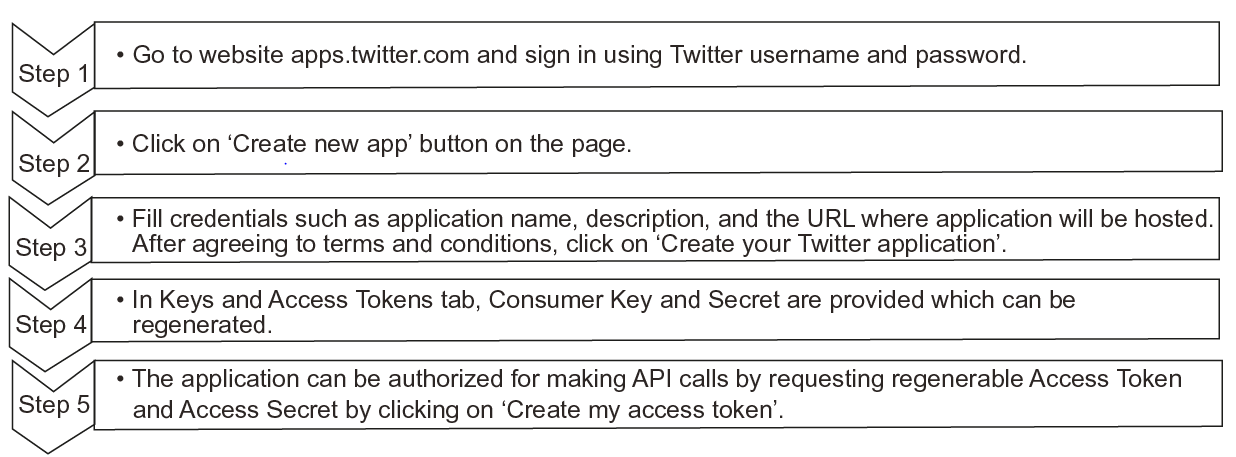
\includegraphics{1.png}

    \subsection{ Collecting User's Information
}\label{collecting-users-information}

    \begin{Verbatim}[commandchars=\\\{\}]
{\color{incolor}In [{\color{incolor}1}]:} \PY{k+kn}{import} \PY{n+nn}{tweepy}
        
        \PY{k}{def} \PY{n+nf}{OAuthVerifier}\PY{p}{(}\PY{p}{)}\PY{p}{:}
            \PY{l+s+sd}{\PYZsq{}\PYZsq{}\PYZsq{}}
        \PY{l+s+sd}{    Objective: To authorize the application to access Twitter}
        \PY{l+s+sd}{    Input Parameter: None}
        \PY{l+s+sd}{    Return Value: API object}
        \PY{l+s+sd}{    \PYZsq{}\PYZsq{}\PYZsq{}}
            \PY{n}{consumerKey} \PY{o}{=} \PY{l+s+s1}{\PYZsq{}}\PY{l+s+s1}{iym0XRG0SOgyPOjmlPQgB4XrC}\PY{l+s+s1}{\PYZsq{}}
            \PY{n}{consumerSecret} \PY{o}{=} \PY{l+s+s1}{\PYZsq{}}\PY{l+s+s1}{I6gBj8RpcXJvN6xaKUUGeTkPEDpHziRXBmT9d9yG8k5Ik0H0bF}\PY{l+s+s1}{\PYZsq{}}
            \PY{n}{authorization} \PY{o}{=} \PY{n}{tweepy}\PY{o}{.}\PY{n}{OAuthHandler}\PY{p}{(}\PY{n}{consumerKey}\PY{p}{,} \PY{n}{consumerSecret}\PY{p}{)}
            \PY{n}{accessToken} \PY{o}{=} \PY{l+s+s1}{\PYZsq{}}\PY{l+s+s1}{727494459118653446\PYZhy{}XWf9MmBJmCUOM7Ic9xvoHlZCBQAWWA1}\PY{l+s+s1}{\PYZsq{}}
            \PY{n}{accessSecret} \PY{o}{=} \PY{l+s+s1}{\PYZsq{}}\PY{l+s+s1}{jl4UJPXYSC8ygV8EsyNz6fMOW2NEs9NFvJc2InyfXNvve}\PY{l+s+s1}{\PYZsq{}}
            \PY{n}{authorization}\PY{o}{.}\PY{n}{set\PYZus{}access\PYZus{}token}\PY{p}{(}\PY{n}{accessToken}\PY{p}{,} \PY{n}{accessSecret}\PY{p}{)}
            \PY{n}{api} \PY{o}{=} \PY{n}{tweepy}\PY{o}{.}\PY{n}{API}\PY{p}{(}\PY{n}{authorization}\PY{p}{)}
            \PY{k}{return} \PY{n}{api}
        
        \PY{k}{def} \PY{n+nf}{getUserStatistics}\PY{p}{(}\PY{n}{user}\PY{p}{)}\PY{p}{:}
            \PY{l+s+sd}{\PYZsq{}\PYZsq{}\PYZsq{}}
        \PY{l+s+sd}{    Objective: To get user statistics using various}
        \PY{l+s+sd}{            variables of the api}
        \PY{l+s+sd}{    Input Parameter: user \PYZhy{} string}
        \PY{l+s+sd}{    Return Value: None}
        \PY{l+s+sd}{    \PYZsq{}\PYZsq{}\PYZsq{}}
            \PY{n+nb}{print}\PY{p}{(}\PY{l+s+s1}{\PYZsq{}}\PY{l+s+se}{\PYZbs{}n}\PY{l+s+s1}{Name: }\PY{l+s+s1}{\PYZsq{}}\PY{p}{,} \PY{n}{user}\PY{o}{.}\PY{n}{name}\PY{p}{)}
            \PY{n+nb}{print}\PY{p}{(}\PY{l+s+s1}{\PYZsq{}}\PY{l+s+s1}{Screen Name: }\PY{l+s+s1}{\PYZsq{}}\PY{p}{,} \PY{n}{user}\PY{o}{.}\PY{n}{screen\PYZus{}name}\PY{p}{)}
            \PY{n+nb}{print}\PY{p}{(}\PY{l+s+s1}{\PYZsq{}}\PY{l+s+s1}{ID: }\PY{l+s+s1}{\PYZsq{}}\PY{p}{,} \PY{n}{user}\PY{o}{.}\PY{n}{id}\PY{p}{)}
            \PY{n+nb}{print}\PY{p}{(}\PY{l+s+s1}{\PYZsq{}}\PY{l+s+s1}{Account creation date and time: }\PY{l+s+s1}{\PYZsq{}}\PY{p}{,} \PY{n}{user}\PY{o}{.}\PY{n}{created\PYZus{}at}\PY{p}{)}
            \PY{n+nb}{print}\PY{p}{(}\PY{l+s+s1}{\PYZsq{}}\PY{l+s+s1}{Location: }\PY{l+s+s1}{\PYZsq{}}\PY{p}{,} \PY{n}{user}\PY{o}{.}\PY{n}{location}\PY{p}{)}
            \PY{n+nb}{print}\PY{p}{(}\PY{l+s+s1}{\PYZsq{}}\PY{l+s+s1}{Description: }\PY{l+s+s1}{\PYZsq{}}\PY{p}{,} \PY{n}{user}\PY{o}{.}\PY{n}{description}\PY{p}{)}
            \PY{n+nb}{print}\PY{p}{(}\PY{l+s+s1}{\PYZsq{}}\PY{l+s+s1}{No. of followers: }\PY{l+s+s1}{\PYZsq{}}\PY{p}{,} \PY{n}{user}\PY{o}{.}\PY{n}{followers\PYZus{}count}\PY{p}{)}
            \PY{n+nb}{print}\PY{p}{(}\PY{l+s+s1}{\PYZsq{}}\PY{l+s+s1}{No. of friends: }\PY{l+s+s1}{\PYZsq{}}\PY{p}{,} \PY{n}{user}\PY{o}{.}\PY{n}{friends\PYZus{}count}\PY{p}{)}
            \PY{n+nb}{print}\PY{p}{(}\PY{l+s+s1}{\PYZsq{}}\PY{l+s+s1}{No. of favourite tweets: }\PY{l+s+s1}{\PYZsq{}}\PY{p}{,} \PY{n}{user}\PY{o}{.}\PY{n}{favourites\PYZus{}count}\PY{p}{)}
            \PY{n+nb}{print}\PY{p}{(}\PY{l+s+s1}{\PYZsq{}}\PY{l+s+s1}{No. of posted tweets: }\PY{l+s+s1}{\PYZsq{}}\PY{p}{,} \PY{n}{user}\PY{o}{.}\PY{n}{statuses\PYZus{}count}\PY{p}{)}
            \PY{n+nb}{print}\PY{p}{(}\PY{l+s+s1}{\PYZsq{}}\PY{l+s+s1}{Associated URL: }\PY{l+s+s1}{\PYZsq{}}\PY{p}{,} \PY{n}{user}\PY{o}{.}\PY{n}{url}\PY{p}{)}
        
        \PY{k}{def} \PY{n+nf}{main}\PY{p}{(}\PY{p}{)}\PY{p}{:}
            \PY{l+s+sd}{\PYZsq{}\PYZsq{}\PYZsq{}}
        \PY{l+s+sd}{    Objective: To collect user information}
        \PY{l+s+sd}{    Input Parameter: None}
        \PY{l+s+sd}{    Return Value: None}
        \PY{l+s+sd}{    \PYZsq{}\PYZsq{}\PYZsq{}}
            \PY{c+c1}{\PYZsh{} To print user\PYZsq{}s information}
            \PY{n}{api} \PY{o}{=} \PY{n}{OAuthVerifier}\PY{p}{(}\PY{p}{)}
            \PY{c+c1}{\PYZsh{} Authenticated User}
            \PY{n}{user} \PY{o}{=} \PY{n}{api}\PY{o}{.}\PY{n}{me}\PY{p}{(}\PY{p}{)}
            \PY{n}{getUserStatistics}\PY{p}{(}\PY{n}{user}\PY{p}{)}
        
        \PY{k}{if} \PY{n+nv+vm}{\PYZus{}\PYZus{}name\PYZus{}\PYZus{}} \PY{o}{==} \PY{l+s+s1}{\PYZsq{}}\PY{l+s+s1}{\PYZus{}\PYZus{}main\PYZus{}\PYZus{}}\PY{l+s+s1}{\PYZsq{}}\PY{p}{:}
            \PY{n}{main}\PY{p}{(}\PY{p}{)}
\end{Verbatim}


    \begin{Verbatim}[commandchars=\\\{\}]

Name:  Suzzane Mathew
Screen Name:  SuzzaneMathew
ID:  727494459118653446
Account creation date and time:  2016-05-03 13:46:10
Location:  India
Description:  A Python Programmer
No. of followers:  4
No. of friends:  34
No. of favourite tweets:  0
No. of posted tweets:  3
Associated URL:  None

    \end{Verbatim}

    \subsection{ Collecting Tweets Having Specific Words
}\label{collecting-tweets-having-specific-words}

    \begin{itemize}
\item
  \textbf{StreamListener class}: used for collecting streaming tweets.
\item
  Class MyStreamListener inherits the class StreamListener of the tweepy
  module.
\item
  In the class MyStreamListener, we define two methods: on\_status and
  on\_error.

\begin{verbatim}
* The method on_status tells what to do when a status (input parameter) 
  known as tweet update is received.  
* The method on_error handles the error and gets automatically invoked
  on occurrence of an error.
\end{verbatim}
\end{itemize}

    \begin{Verbatim}[commandchars=\\\{\}]
{\color{incolor}In [{\color{incolor} }]:} \PY{k+kn}{import} \PY{n+nn}{tweepy}
        
        
        \PY{k}{class} \PY{n+nc}{MyStreamListener}\PY{p}{(}\PY{n}{tweepy}\PY{o}{.}\PY{n}{StreamListener}\PY{p}{)}\PY{p}{:}
            \PY{c+c1}{\PYZsh{} Class inheriting StreamListener of tweepy module}
        
            \PY{k}{def} \PY{n+nf}{on\PYZus{}status}\PY{p}{(}\PY{n+nb+bp}{self}\PY{p}{,} \PY{n}{status}\PY{p}{)}\PY{p}{:}
                \PY{l+s+sd}{\PYZsq{}\PYZsq{}\PYZsq{}}
        \PY{l+s+sd}{        Objective: To print text stream of tweets}
        \PY{l+s+sd}{        Input Parameters:}
        \PY{l+s+sd}{            self (implicit parameter) \PYZhy{} object of type}
        \PY{l+s+sd}{            MyStreamListener}
        \PY{l+s+sd}{            status \PYZhy{} string value representing tweet}
        \PY{l+s+sd}{        Return Value: None}
        \PY{l+s+sd}{        \PYZsq{}\PYZsq{}\PYZsq{}}
                \PY{n+nb}{print}\PY{p}{(}\PY{n}{status}\PY{o}{.}\PY{n}{text}\PY{p}{)}
            
            \PY{k}{def} \PY{n+nf}{on\PYZus{}error}\PY{p}{(}\PY{n+nb+bp}{self}\PY{p}{,} \PY{n}{status}\PY{p}{)}\PY{p}{:}
                \PY{l+s+sd}{\PYZsq{}\PYZsq{}\PYZsq{}}
        \PY{l+s+sd}{        Objective: To disconnect the stream by returning False}
        \PY{l+s+sd}{        if error 420 occurs}
        \PY{l+s+sd}{        Input Parameters:}
        \PY{l+s+sd}{            self (implicit parameter) \PYZhy{} object of type}
        \PY{l+s+sd}{            MyStreamListener}
        \PY{l+s+sd}{            status \PYZhy{} int value representing error code}
        \PY{l+s+sd}{        Return Value: result \PYZhy{} int}
        \PY{l+s+sd}{        \PYZsq{}\PYZsq{}\PYZsq{}}
                \PY{k}{if} \PY{n}{status}\PY{o}{==}\PY{l+m+mi}{420}\PY{p}{:}
                    \PY{k}{return} \PY{k+kc}{False}
        
        \PY{k}{def} \PY{n+nf}{main}\PY{p}{(}\PY{p}{)}\PY{p}{:}
            \PY{l+s+sd}{\PYZsq{}\PYZsq{}\PYZsq{}}
        \PY{l+s+sd}{    Objective: To print streaming data containing given keywords}
        \PY{l+s+sd}{    Input Parameter: None}
        \PY{l+s+sd}{    Return Value: None}
        \PY{l+s+sd}{    \PYZsq{}\PYZsq{}\PYZsq{}}
            \PY{n}{api} \PY{o}{=} \PY{n}{OAuthVerifier}\PY{p}{(}\PY{p}{)}
            \PY{c+c1}{\PYZsh{} Creates a stream listener object listenerOb}
            \PY{n}{listenerOb} \PY{o}{=} \PY{n}{MyStreamListener}\PY{p}{(}\PY{p}{)}
            \PY{c+c1}{\PYZsh{} Create a Stream object}
            \PY{n}{myStream} \PY{o}{=} \PY{n}{tweepy}\PY{o}{.}\PY{n}{Stream}\PY{p}{(}\PY{n}{api}\PY{o}{.}\PY{n}{auth}\PY{p}{,} \PY{n}{listenerOb}\PY{p}{)}
            \PY{c+c1}{\PYZsh{} Starts streaming by specifying search keywords}
            \PY{n}{searchList} \PY{o}{=} \PY{n+nb}{eval}\PY{p}{(}\PY{n+nb}{input}\PY{p}{(}\PY{l+s+s1}{\PYZsq{}}\PY{l+s+s1}{Enter search keywords list: }\PY{l+s+s1}{\PYZsq{}}\PY{p}{)}\PY{p}{)}
            \PY{n}{myStream}\PY{o}{.}\PY{n}{filter}\PY{p}{(}\PY{n}{track} \PY{o}{=} \PY{n}{searchList}\PY{p}{)}
        
        \PY{k}{if} \PY{n+nv+vm}{\PYZus{}\PYZus{}name\PYZus{}\PYZus{}} \PY{o}{==} \PY{l+s+s1}{\PYZsq{}}\PY{l+s+s1}{\PYZus{}\PYZus{}main\PYZus{}\PYZus{}}\PY{l+s+s1}{\PYZsq{}}\PY{p}{:}
            \PY{n}{main}\PY{p}{(}\PY{p}{)}
\end{Verbatim}


    \begin{Verbatim}[commandchars=\\\{\}]
Enter search keywords list: ['Python','Programming']
RT: Forest Edge ES \#ForestEdgeES \#Elementary \#School for \#Robotics \#Programming at Royal Cyber Club 🕰️🖥️🎮💎 https://t.co/06PXj3zDVz
RT: Sunrise Valley ES \#SunriseValleyES \#Elementary \#School for \#Robotics \#Programming at Royal Cyber Club 🕰️🖥️🎮💎 https://t.co/kaZ8da8O3W
RT @LoharPrasanna: Which Programming language should you learn ? https://t.co/WcwhuGg4Q8
2 дня начал читать книгу Бьерна Страуструпа - Язык программирования С++

\#обучение \#Programming \#cplusplus
Diet-Microbiota Interactions Mediate Global Epigenetic Programming in Multiple Host Tissues - ScienceDirect https://t.co/rkr0yQAIYt
RT: Daniels Run ES \#DanielsRunES \#Elementary \#School for 3D Game Programming (1-6th Grade) @ STEM Summer Camp 🕰️🖥️🎮💎 https://t.co/zhtoL7VFoi
RT: Clearview ES \#ClearviewES \#Elementary \#School for 3D Game Programming (1-6th Grade) @ STEM Summer Camp 🕰️🖥️🎮💎 https://t.co/XO9gHDDWYD
@python NowTime: 2018/03/17 03:09:23.3863
TweetCount: 319
RT: Cub Run ES \#CubRunES \#Elementary \#School for \#Robotics \#Programming at Royal Cyber Club 🕰️🖥️🎮💎 https://t.co/DklLcyeYv8
RT @sensitiveemmett: i know people don't like daylight savings time because it screws up their sleep schedules, but *nothing* will make you…
The Top 9 Technology of 2016  \#javascript \#Python https://t.co/dPgXc3pcHe
RT @DIBIADream: DREAM is proud to present our 2017 Impact \&amp; Initiatives Report. Continuing to spark social change through programming that…
Zigbee Showcased at CES2017 Path to Unified.. \#programming \#麻雀の役 https://t.co/iGxjc8RHzh
RT @allen\_data: Python GUI Programming using Tkinter and Python 3

☞ https://t.co/UZktnwixdN

\#hadoop \#spark https://t.co/WYZ4mXuOc5
RT @TheBrando2: Monty Python and the Holy Grail (1975) https://t.co/purMRtV0vJ
Global IIoT Technologies, Solutions{\ldots} \#programming \#麻雀の役 https://t.co/RBuRZjmjrz
Connectivity Foundation and AllSeen Alliance Team up{\ldots} \#javascript \#Python https://t.co/sEn4UHvDvL
Immediate Availability of ConnectCore for i.MX6UL Starter Kit..  \#javascript \#Python https://t.co/3z4oiMAFDE
RT @enthought: You used to write \#python like C code{\ldots} @LEGOWorldsGame https://t.co/0hVNLd96IS
John Cleese taking a break on the set of Monty Python and the Holy Grail (1975) https://t.co/YHdUzCU1fZ
VMs look to edge out gateways in push..  \#javascript \#Python https://t.co/oWB0OqapuA
RT: Fairfax Community Church for \#Programming cool games \#STEMCamps \#Kids \#Education 🕰️🖥️🎮💎 https://t.co/ly6NIjOtzo
RT: Fairfax Presbyterian Church for \#STEM \#Classes \#Designing \#Legos \#Programming \#Modeling \#Kids \#Education 🕰️🖥️🎮💎 https://t.co/aAte8smBO7
CVproof will connect with HR groups specifically and additionally through associations with real Human Resources In… https://t.co/6DF8SR7u8I
RT: Centreville Presbyterian Church for \#STEM \#Classes \#Designing \#Legos \#Programming \#Modeling \#Kids \#Education 🕰️… https://t.co/TMIV88fEqE
RT: Korean Central Presbyterian for \#Robotics \#Programming \#Modeling \#STEMCamps \#Kids \#Education 🕰️🖥️🎮💎 https://t.co/TBomMLVkNP
Public libraries invited to apply for ‘The Great American Read’ PBS programming grants
https://t.co/oSzqpIxd0r
RT @elpais\_cultura: Dice el ex Monty Python que sus integrantes son como la muchedumbre que asalta con antorchas el castillo de Frankenstei…
RT: Centreville Farms Community Association for \#Robotics \#Programming \#Modeling \#STEMCamps \#Kids \#Education 🕰️🖥️🎮💎 https://t.co/hNctx6BRj5
Programming Alert: Boxing promoter \#DonKing joins @cvpayne to discuss he state of boxing as a sport and a business… https://t.co/0Vg5DWEmUx
RT: Pat White Center at Ben Lomond for \#STEM \#Classes \#Designing \#Legos \#Programming \#Modeling \#Kids \#Education 🕰️… https://t.co/HE46FGj1M2
RT: Church of the Good Shepherd for \#Programming cool games \#STEMCamps \#Kids \#Education 🕰️🖥️🎮💎 https://t.co/JwHeR0DLAm
RT @Robzmob: \#FridayMotivation ; ) They have \#Programming . . , but we have \#Brains !! \#TheStormIsHere !! \#WeThePeople are \#BrainSTORMing t…
RT: Stenwood ES \#StenwoodES \#Elementary \#School for 3D Game Programming (1-6th Grade) @ STEM Summer Camp 🕰️🖥️🎮💎 https://t.co/0XZhaHptpr
RT @FoxBusiness: Programming Alert: Boxing promoter \#DonKing joins @cvpayne to discuss he state of boxing as a sport and a business and his…
Which are the most popular programming languages at hackathons? \#hackathon \#javascript \#reactjs \#nodejs
https://t.co/Z8R1xAKGAl
How to run \#Capybara feature specs with \#Selenium and headless \#Chrome \#ruby \#rails \#rubyonrails \#bosnia… https://t.co/fSCX3KdxqA
Do you have Python 2 code that urgently needs to get migrated to Python 3? Just @anthonypjshaw and me on episode 15… https://t.co/K8SrKrSboP
RT @JRLibrarian: As requested - here are four weeks of programming ideas and activities reflecting weekly AASL School Library Month subthem…
RT @Hakin9: A Practical Introduction to Blockchain with Python https://t.co/fwmWjrPH3a \#infosec \#hacking \#hackers… https://t.co/CBAP5wQtWX
RT @feminnazty: Yo shut up I remember losing a whole day of programming cause Nickelodeon wanted us to exercise 
Ya kids will live while 17…
STMicroelectronics Innovative.. \#programming \#麻雀の役  https://t.co/lV66oc9FyD
New World of Intelligent Devices..  \#programming \#麻雀の役 https://t.co/c0xE9qxHqi
RT @CodeWisdom: "Programming is the art of algorithm design and the craft of debugging errant code." - Ellen Ullman
RT: Center Ridge Region Home Owner for \#Robotics \#Programming Educational Classes For Kids 🕰️🖥️🎮💎 https://t.co/Aw5oWF817J
RT @DuncanGalbrait1: Monty Python - Life of Brian - PFJ Union meeting https://t.co/jVlH3BdUSW via @YouTube
Commercial Craft Brewing Appliances for{\ldots} \#programming \#麻雀の役 https://t.co/9p9GGYiFzS
RT: Chantilly Highlands Community for \#STEM \#Classes \#Designing \#Legos \#Programming \#Modeling \#Kids \#Education 🕰️🖥️… https://t.co/u36iqr6wi7
RT @WWEGraves: I’m terribly sorry that your parents didn’t love you enough. Here is some of the attention you so desperately seek. (Just ma…
RT @abubakar47i: It mobilizes the smartest minds from \&gt;100 countries to apply their business thinking to solve world’s most pressing issues…
RT @KirkDBorne: Programming Languages for \#DataScience and \#MachineLearning (with samples of source code) https://t.co/s7RyNXwC7H \#abdsc \#B…
RT: London Towne ES \#LondonTowneFCPS \#Elementary \#School for \#Robotics \#Programming at Royal Cyber Club 🕰️🖥️🎮💎 https://t.co/afiy2FZfOz
RT @jeremynewberger: .@SeanHannity and @IngrahamAngle scolding @ShepNewsTeam on how newsy their programs are is like Joel Steinberg and Hed…
@python NowTime: 2018/03/17 03:10:33.7043
TweetCount: 321
RT: Stacy C. Sherwood Community Center for \#Robotics \#Programming Educational Classes For Kids 🕰️🖥️🎮💎 https://t.co/eqDEl0WXpo
Practical Python Data Science Techniques

☞ https://t.co/wRehxtDtxn

\#bigdata https://t.co/eC9H5UTA65
RT @lucasoft\_co\_uk: RT @Hakin9: A Practical Introduction to Blockchain with Python https://t.co/fwmWjrPH3a \#infosec \#hacking \#hackers \#pent…
RT: Brookfield ES \#BrookfieldES \#Elementary for \#Programming \#MinecraftModding at Royal Cyber Club 🕰️🖥️🎮💎 https://t.co/lSMgfadcED
RT: Herndon ES \#Herndon\_ES \#Elementary \#School for 3D Game Programming (1-6th Grade) @ STEM Summer Camp 🕰️🖥️🎮💎 https://t.co/qBiA3hYugu
RT: Herndon Community Center for \#Robotics \#Programming \#Modeling \#STEMCamps \#Kids \#Education 🕰️🖥️🎮💎 https://t.co/yX99sLWmNj
RT: Grace Covenant Church for \#Robotics \#Programming \#Modeling \#STEMCamps \#Kids \#Education 🕰️🖥️🎮💎 https://t.co/0RXTSlXTWj
RT: Centreville Community Church for \#Robotics \#Programming Educational Classes For Kids 🕰️🖥️🎮💎 https://t.co/SNlXTMuvAJ
Yay for cool graphs and charts in your reports! https://t.co/8Mgyx6yymE
RT: Grace Covenant Church for \#Programming cool games \#STEMCamps \#Kids \#Education 🕰️🖥️🎮💎 https://t.co/7JoxuYahQh
@IngrahamAngle No he is right. Your programming is illlegit propaganda
RT: Greenbriar Community Center for \#Robotics \#Programming Educational Classes For Kids 🕰️🖥️🎮💎 https://t.co/ethUZhby6u
RT @FoxBusiness: Programming Alert: Peter Thiel sits down with @MariaBartiromo for an exclusive interview on @MorningsMaria - Friday 7a ET…
RT @FoxBusiness: Programming Alert: Boxing promoter \#DonKing joins @cvpayne to discuss he state of boxing as a sport and a business and his…
\#OpenGL \#Programming \#Math \#Matrix \#CPP \#Developers \#GLSL Reminder: your regular modelview (MV) matrix may squish y… https://t.co/eWGg0cIqKb
RT: Lord of Life Lutheran Church for \#Robotics \#Programming Educational Classes For Kids 🕰️🖥️🎮💎 https://t.co/6UCY9ZI8Sq
RT: Centreville Presbyterian Church for \#STEM \#Classes \#Designing \#Legos \#Programming \#Modeling \#Kids \#Education 🕰️… https://t.co/QMWJQ5elDi
RT @ReaktorNow: Together with @helsinkiuni we are developing a free online course called the Elements of AI. The course requires no program…
RT @SecurityTube: Python for Pentesters: Directory Navigation https://t.co/8yaK0A4TO9 https://t.co/9eLe8yRcbj
RT: Daniels Run ES \#DanielsRunES \#Elementary \#School for 3D Game Programming (1-6th Grade) @ STEM Summer Camp 🕰️🖥️🎮💎 https://t.co/6Ko3L8GkC1
RT @Aly\_Raisman: Please join the effort to address sexual abuse in sport. I have partnered with Darkness 2 Light to make programming availa…
QISKit: quantum computing with python https://t.co/ut0D9Sbrv6 via @IBMCode
RT: Center Ridge Region Home Owner for \#Robotics \#Programming \#Modeling \#STEMCamps \#Kids \#Education 🕰️🖥️🎮💎 https://t.co/Vc9gzBCu0r
RT: Aldrin ES \#AldrinEagles \#Elementary \#School for 3D Game Programming (1-6th Grade) @ STEM Summer Camp 🕰️🖥️🎮💎 https://t.co/FEMwjW1EWd
RT @Mason9780: New technology is now making it possible for viewers to record and store high definition programming onto DVDs. https://t.co…
RT @christi3k: I'm looking for my next gig as a software engineer or developer advocate in Portland, OR, or remote (preferred)! I'm an expe…
RT: Centreville Baptist Church for \#Robotics \#Programming Educational Classes For Kids 🕰️🖥️🎮💎 https://t.co/cFmMkR8m5p
RT @FoxBusiness: Programming Alert: Boxing promoter \#DonKing joins @cvpayne to discuss he state of boxing as a sport and a business and his…
Comienza \#BetaBeersODB con @JAR\_omero hablándonos de Django \#python https://t.co/FfQgR8R7cA
Over 1600 students in 22 programs{\ldots} 75 in \#engineering{\ldots} plus 100\% of last year's welding grads were called by pr… https://t.co/rpoksKVqlh
I'm excited to attend "Using Scratch Programming to Teach World Language" at CABE 2018. Come with me?… https://t.co/lh2ddz5TSc
RT: Sully Station Community Center for \#Robotics \#Programming Educational Classes For Kids 🕰️🖥️🎮💎 https://t.co/umxEB1e0B8
RT: Powell ES \#ColinPowellES \#Elementary \#School for \#Robotics \#Programming at Royal Cyber Club 🕰️🖥️🎮💎 https://t.co/QHoF8MLLmv
RT @Hakin9: A Practical Introduction to Blockchain with Python https://t.co/m8vK9WUzHU \#infosec \#hacking \#hackers \#pentesting \#pentest \#pro…
RT: Centreville Community Church for \#STEM \#Classes \#Designing \#Legos \#Programming \#Modeling \#Kids \#Education 🕰️🖥️🎮💎 https://t.co/GShZ7YHdcu
RT @svpersof: Hello everyone! I got accepted into my study abroad program to learn about international healthcare \&amp; public health in Japan.…
RT @FoxBusiness: Programming Alert: Boxing promoter \#DonKing joins @cvpayne to discuss he state of boxing as a sport and a business and his…
RT @KitPloit: Powershell-RAT - Python Based Backdoor That Uses Gmail To Exfiltrate Data Through Attachment https://t.co/WubR2u62o5 \#Backdoo…
@mia\_0327 https://t.co/oopF1g9ThH
ちなみにあのポコポコのやろうとしてた元ネタはコレで。そしてやってて気づいたのが……方式が間違っていた……今の方法じゃこれは作れない……やり直しだ……!
で現在ソース書き直し中。
RT: Aldrin ES \#AldrinEagles \#Elementary for \#Programming \#MinecraftModding at Royal Cyber Club 🕰️🖥️🎮💎 https://t.co/t9NXCydeFJ
RT @chris\_\_martin: The "domain object" pattern was one of the most destructive forces at my first programming job. We'd write *one* Java cl…
RT: Floris United Methodist Church for \#STEM \#Classes \#Designing \#Legos \#Programming \#Modeling \#Kids \#Education 🕰️… https://t.co/KDgfAJkvI6
RT @mocityschool: Did you see @TheSpec article about our Intro to Construction 🚧 for Women 👷🏽‍♀️course with @EvaRothwell460 @ONTrillium tod…
RT: Clearview ES \#ClearviewES \#Elementary for \#Programming \#MinecraftModding at Royal Cyber Club 🕰️🖥️🎮💎 https://t.co/bratpnvqBo
RT: Daniels Run ES \#DanielsRunES \#Elementary \#School for 3D Game Programming (1-6th Grade) @ STEM Summer Camp 🕰️🖥️🎮💎 https://t.co/bsQ3RrwjQC
RT @WWEGraves: I’m terribly sorry that your parents didn’t love you enough. Here is some of the attention you so desperately seek. (Just ma…
RT @BigDataFr\_: ✔️ Offre de Stage HPC Ingénieur/Bac+5 Maths-Info
•Cuda, Python, NumPy, Scikit-Learn, Keras, Caffe,… https://t.co/z4ex4T1KRA
https://t.co/meDjQfnVam [ Programming \&amp; Design ] Open Question : SQL database in trouble? \#yahooanswers \#questions \#answers
fun time remote pair programming to practice C++ TDD 
with a @TKPJava graduate https://t.co/0uzn8r2aOS
@python NowTime: 2018/03/17 03:11:44.773
TweetCount: 323
RT: Sully Station Community Center for \#Robotics \#Programming Educational Classes For Kids 🕰️🖥️🎮💎 https://t.co/OUBtki1fah
This is going to strangle entrepreneurs and small sellers. A \$12 Etsy sale will now not only have to charge shippin… https://t.co/l01GTegh7z
The new Conditional Types capabilities in @typescriptlang 2.8 move the language even more firmly into type-level pr… https://t.co/2ElyZI5Mxc
RT: Virginia Run ES \#VirginiaRunES \#Elementary for \#Programming \#MinecraftModding at Royal Cyber Club 🕰️🖥️🎮💎 https://t.co/xfIuUhc9bG
RT @FoxBusiness: Programming Alert: Boxing promoter \#DonKing joins @cvpayne to discuss he state of boxing as a sport and a business and his…
We're at a standstill at work because my boss's boss never gives us a programming budget and just tells us vague id… https://t.co/lgYz64VpWu
RT: Crossfield ES \#CrossfieldES \#Elementary for \#Programming \#MinecraftModding at Royal Cyber Club 🕰️🖥️🎮💎 https://t.co/CnE5Gjk7ta
RT: Greenbriar Community Center for \#Robotics \#Programming \#Modeling \#STEMCamps \#Kids \#Education 🕰️🖥️🎮💎 https://t.co/uP5wOlUood
Excellent! Thanks for PRIMM-ing!! @KingsECS https://t.co/2QjyawHVU4
Canterbury Woods ES \#Canterbury\_Wood \#Elementary \#School for 3D Game Programming (1-6th) @ STEM Summer Camp 🕰️🖥️🎮💎 https://t.co/d6kxwWBjFH
RT @gethackteam: Which are the most popular programming languages at hackathons? \#hackathon \#javascript \#reactjs \#nodejs
https://t.co/Z8R1x…
RT: Summer Camp registration is open! STEM, Minecraft, Robotics, Game Design, Game Programming! 🆒 🌞 🕰️ https://t.co/vmLyRcifDq
@JDM1114 \&amp; @GregHughesNBCSG You guys are better than this, right? If not, we can help. \#sunsetNBC… https://t.co/17b1zBKxZh
RT @saeedamenfx: the master of Python @dyjh speaking! Great talk, always learn something new from Yves! \#WBS @QuantsHub https://t.co/vWj5K8…
Real Good Community Programming only on 91.1 The Bridge! https://t.co/2mQ6K9uLw2 on \#Podbean
Real Good Community Programming only on 91.1 The Bridge! https://t.co/qs54crPbj5 on \#Podbean
Real Good Community Programming only on 91.1 The Bridge! https://t.co/R6Qzg2fYaz on \#Podbean
RT @lucasoft\_co\_uk: RT @Hakin9: A Practical Introduction to Blockchain with Python https://t.co/fwmWjrPH3a \#infosec \#hacking \#hackers \#pent…
RT @WWEGraves: I’m terribly sorry that your parents didn’t love you enough. Here is some of the attention you so desperately seek. (Just ma…
Thanks for having us! https://t.co/CJTJfpVhHd
I wish I had more people to work out with. I love seeing different people's programming and goals.
RT: \#STEM \#Robotics \#Programming \#Modeling \#STEMCamps \#Kids \#Education 🕰️🖥️🎮💎 at Royal Cyber Club https://t.co/bkcvpn4vQD
RT @WWEGraves: I’m terribly sorry that your parents didn’t love you enough. Here is some of the attention you so desperately seek. (Just ma…
RT @LorenaABarba: I'm making an open online course with the first module of our computing course for engineers—Get Data Off The Ground with…
RT @jcldf: Python based backdoor that uses Gmail to exfiltrate data as an e-mail attachment.

This RAT will help someone during red team en…
Por isso que eu digo que os caras do Monty Python eram gênios. https://t.co/vT7uGGUxmh
I know I complain a lot, and freak out a lot, but let me first say that I am blessed to have a support system in my… https://t.co/wlepj90nmY
RT: Poplar Tree ES \#PoplarTreeES \#Elementary \#School for \#Robotics \#Programming at Royal Cyber Club 🕰️🖥️🎮💎 https://t.co/JQ8PgWWJaj
Practical Python Data Science Techniques

☞ https://t.co/ndqjsgz0pp

\#bigdata https://t.co/54gkBmNjMD
RT @CodeWisdom: "Everyday life is like programming, I guess. If you love something you can put beauty into it." - Donald Knuth
RT @SecurityTube: Python for Pentesters: Directory Navigation https://t.co/8yaK0A4TO9 https://t.co/9eLe8yRcbj
RT @dustmop: Hi! I'm a full-stack / backend freelance engineer looking for part-time contract work. C++, go, node.js, python, and more. Enj…
RT @mlemweb: Our Digital Humanities Workshop is tomorrow! @dustyweb and I are finalizing our tutorials now. We've still got some spaces lef…
RT: Southgate Community Center for \#Robotics \#Programming \#Modeling \#STEMCamps \#Kids \#Education 🕰️🖥️🎮💎 https://t.co/fX4QnlWfqK
Our Education Program partners with Inwater Research Group to promote quality educational programming. The{\ldots} https://t.co/nLCx32kl7P
RT @TalkPython: Do you have Python 2 code that urgently needs to get migrated to Python 3? Just @anthonypjshaw and me on episode 155 of @ta…
RT: Aldrin ES \#AldrinEagles \#Elementary \#School for \#Robotics \#Programming at Royal Cyber Club 🕰️🖥️🎮💎 https://t.co/IFf5v1mYMT
@briangcronin That's the main ingredient to making great programming videos -- great content and great explanations… https://t.co/eWweUZL9SA
RT @Onitaset: New working theme: "Today we will discuss how you are failing Black people and what you need to do to change that.  . . . 99\%…
RT @WWEGraves: I’m terribly sorry that your parents didn’t love you enough. Here is some of the attention you so desperately seek. (Just ma…
RT @jdmorenob: ¡Diario Lenguajes de programación! https://t.co/RE7n2nBgni \#in Gracias a @danielriveraaya @galilea\_ti @iconsolutions14 \#php…
Join Jules Damji (@2twitme) @ApacheSpark \&amp; Community Advocate at @Databricks to learn how to jumpstart writing cont… https://t.co/0K6MoQY6bB
RT @mlemweb: Our Digital Humanities Workshop is tomorrow! @dustyweb and I are finalizing our tutorials now. We've still got some spaces lef…
RT: Reston Community Center for \#STEM \#Classes \#Designing \#Legos \#Programming \#Modeling \#Kids \#Education 🕰️🖥️🎮💎 https://t.co/q1nMZB53Su
@scuttlingvoid prob a piebald ball python ye !!
i always feel so powerful learning programming but then one mistake happens that wrecks all my code and I turn into a slimy ball of bad
RT @ReaktorNow: Together with @helsinkiuni we are developing a free online course called the Elements of AI. The course requires no program…
I just liked “Introduce 'JS Weight tracer' Python Effector” by @oinon on \#Vimeo: https://t.co/20xorZvGXu
@\_\_Zanele Oh no. 😷 Imagine being a python just nje. 😂
For even more \#Python training, come to my sessions at \#FedGIS next week! https://t.co/cV9uUj9UVC
7 Ridicuous Complaints the FCC Received About WWE's Programming https://t.co/Hm39lzhZNp https://t.co/cpKRMrcvvy
Mastering Bitcoin: Programming the Open Blockchain 2nd Edition, (Kindle Edition) https://t.co/rrVJkRu8xT \#text \#yummy \#australianopen
Deciding between a beardie or a ball python is one of the hardest decisions ive ever made
RT: Centreville Community Church for \#STEM \#Robotics \#Programming \#Modeling \#STEMCamps \#Kids \#Education 🕰️🖥️🎮💎 https://t.co/mEq5NYIMsx
Michael Palin is the only good, nice boy from Monty Python
RT: Forest Edge ES \#ForestEdgeES \#Elementary \#School for \#Robotics \#Programming at Royal Cyber Club 🕰️🖥️🎮💎 https://t.co/D4XJpi33h8
RT @CyberToolsBooks: Pro Bash Programming teaches you how to effectively utilize the Ba https://t.co/jCU25KunX2 \#Cybersecurity \#Bitcoin htt…
@annehelen @shannoncoulter That’s been my opinion for a number of years, sadly. It’s really tainted Python for me but oh well.
Modern Serverless Python on Coherence API https://t.co/Hgtsd0Y6ne
Keyword Generator https://t.co/Ic71uaiuFV
@john\_overholt The least known member of Monty Python finally makes headlines. He shoukd have stayed in the shadows.
RT: McNair Farms Community Center for \#Programming cool games \#STEMCamps \#Kids \#Education 🕰️🖥️🎮💎 https://t.co/rZVd73Aeov
RT @WWEGraves: I’m terribly sorry that your parents didn’t love you enough. Here is some of the attention you so desperately seek. (Just ma…
It's the clarity of F\#'s type and function signatures that I miss the most when programming in C\#. https://t.co/iiti5LguvF
@BenedictEvans I do all my programming now off a macbook pro with the touchpad, full screen windows and three finge… https://t.co/E8Y0MxbdYy
RT @RealDebrid: @TeamZT\_ @jsergio123 The guy is just a piece of shit providing a shitty fix then rolling it back assuming we have to comply…
RT @SetonMontessori: Jennifer Nolan contributed a beautiful blog post about our intergenerational programming at Seton Montessori{\ldots} https:…
RT: Reston Community Center for \#STEM \#Robotics \#Programming \#Modeling \#STEMCamps \#Kids \#Education 🕰️🖥️🎮💎 https://t.co/rkZYjjgwqu
RT @abubakar47i: It mobilizes the smartest minds from \&gt;100 countries to apply their business thinking to solve world’s most pressing issues…
えー、pythonのバージョンも落とさないといけないのか
Macromedia Mx Elearning: Advanced Training From The Source  https://t.co/3T2VxqJYJ8 \#Ruby \#programming \#CodingFlux\_
Python Networking: FTP Programming https://t.co/oHutevQjI9
RT @lamifunami: \#SignalsNetwork
Signals is developing a platform for building, training and monetizing crypto trading strategies with a use…
@UKRobotWars I’m sure they’ll fund some educational programming instead, say more baking or talent shows. Come on B… https://t.co/lf7GFXGVdQ
RT: Willow Springs ES \#WSESfox \#Elementary for \#Programming \#MinecraftModding at Royal Cyber Club 🕰️🖥️🎮💎 https://t.co/aFsOvxIHpE
RT: Cherry Run ES \#CherryRunES1 \#Elementary \#School for 3D Game Programming (1-6th Grade) @ STEM Summer Camp 🕰️🖥️🎮💎 https://t.co/Q4Q8C77sme
@1776Stonewall @IngrahamAngle @FoxNews I'm down to @cvpayne \&amp; @LouDobbs {\ldots}thats it for any Fox programming news outlets!
@YYCBoarder @NewWorldHominin @FaithGoldy Invading a country using immigration and neuro linguistic programming word… https://t.co/9Usse9pw9t
বাংলার সব বাঘেরা যখন সিংহকে একসাথে ছোবল দেয়!!  🐅@BCBtigers all players bites like a python! \#BANvSL \#SLvBAN… https://t.co/Fvg0oJ4w88
RT @Hakin9: A Practical Introduction to Blockchain with Python https://t.co/m8vK9WUzHU \#infosec \#hacking \#hackers \#pentesting \#pentest \#pro…
RT @sensitiveemmett: i know people don't like daylight savings time because it screws up their sleep schedules, but *nothing* will make you…
RT: Greenbriar Community Center for \#Programming cool games \#STEMCamps \#Kids \#Education 🕰️🖥️🎮💎 https://t.co/cHuibrW5EM
RT: Little Run ES \#LRroadrunner \#Elementary \#School for 3D Game Programming (1-6th Grade) @ STEM Summer Camp 🕰️🖥️🎮💎 https://t.co/SKg1QdygHz
Most ‘Python’ fans aren’t Trump fans. https://t.co/WVnni846Dj
Why is Python so good for AI and Machine learning?

https://t.co/dwYr04TMiC
@PegCoversTheLaw @steveury Thank you for these midwinter meeting tweets! ABALEL Committee midwinter meetings have g… https://t.co/yDf9SjWbr2
Pandas Cookbook: Recipes For Scientific Computing, Time Series Analysis And Data   https://t.co/DH0sSxUGGj \#python \#programming \#pythonbot\_
RT @SecurityTube: Python for \#Pentesters: Introduction to Python and Setting Up an Environment https://t.co/8yaK0A4TO9  https://t.co/0TPgTC…
@python NowTime: 2018/03/17 03:14:06.045
TweetCount: 327
Introduction to the Python 3 Programming Language - \#python course by @wfbutton https://t.co/XSdfmsXhDm https://t.co/zuQ9loRPCe
RT @FoxBusiness: Programming Alert: Boxing promoter \#DonKing joins @cvpayne to discuss he state of boxing as a sport and a business and his…
RT: Deer Park ES \#DeerParkFCPS \#Elementary \#School for \#Robotics \#Programming at Royal Cyber Club 🕰️🖥️🎮💎 https://t.co/zq9XLaIjxs
High Performance Python: Practical Performant Programming For Humans  https://t.co/3oCq4x44p4 \#python \#flask \#pythonbot\_
@rickathy227 @talace @cheechablunt @Nickelodeon @DLoesch (Someone might want to warn her that Nick has a Go Out and… https://t.co/GZ59KoOS5X
RT @lfcseattle: @JDM1114 \&amp; @GregHughesNBCSG You guys are better than this, right? If not, we can help. \#sunsetNBC \#totaleclipseofthesun \#YN…
RT @fabienLeboeuf: Need to alter Hip joint centre positions of the Conventional Gait Model (\#CGM) with actual position from medical imaging…
@santome7 @thehill Smith is fact based programming. Hannity is opinion based programming. It’s a shame you don’t kn… https://t.co/fFJYg6AbwP
RT @jeffgiesea: ESPN infused its programming with "social justice," ratings declined, and now we learn its CEO was a coke head https://t.co…
RT @CsChapters: Hurry up! Today is the last day to register for @CsharpCorner Gurgaon Chapter Meet to learn \#Python, \#Angular, \#JavaScript,…
RT @ITsax: FPGA-Entwickler / VHDL-Entwickler (m/w) in Freital/Dresden in Freital , \#FPGA \#VHDL \#Informatik \#Python https://t.co/AWYkEt3M1M
RT: Greenbriar Community Center for \#Robotics \#Programming \#Modeling \#STEMCamps \#Kids \#Education 🕰️🖥️🎮💎 https://t.co/A2f97Fmtn4
C/C++ Programming Course Near Sector-72 C and C++ Programming are mu..For more info visit{\ldots} https://t.co/Cf2VXisZqW https://t.co/a0PCZxhdfN
RT: Canterbury Woods ES \#Canterbury\_Wood \#Elementary \#School for 3D Game Programming (1-6th) @ STEM Summer Camp 🕰️… https://t.co/CikRuxlGGC
RT: McNair ES \#FCPSMcNairES \#Elementary for \#Programming \#MinecraftModding at Royal Cyber Club 🕰️🖥️🎮💎 https://t.co/7Vg7gTT77c
RT @RichRogersIoT: Programming is about 13\% math, 15\% theology and the rest is just looking stuff up on the internet - @GonzoHacker
System engineers also do programming.
RT @UPROXX: Netflix has a lovely stockpile of action television programming to binge through. Here's a look at the cream of the crop: https…
RT: Greenbriar Community Center for \#Robotics \#Programming Educational Classes For Kids 🕰️🖥️🎮💎 https://t.co/2Vwj8tQgsb
RT: Korean Central Presbyterian for \#STEM \#Classes \#Designing \#Legos \#Programming \#Modeling \#Kids \#Education 🕰️🖥️🎮💎 https://t.co/3yapfDTrND
\#redfarmers https://t.co/mOef9bxmbR
RT: Powell ES \#ColinPowellES \#Elementary \#School for 3D Game Programming (1-6th Grade) @ STEM Summer Camp 🕰️🖥️🎮💎 https://t.co/UVdpmsxdcb
RT: McNair Farms Community Center for \#Robotics \#Programming \#Modeling \#STEMCamps \#Kids \#Education 🕰️🖥️🎮💎 https://t.co/Ha2ZFuFIOi
@navytheplug Yep, had a couple. 

In church, business, life coach and programming📈
There is a need to integrate climate change issues into the development planning process at all levels, including n… https://t.co/ZYwMDYktok
RT @YourSmartyBro: Python GUI Programming Projects using Tkinter and Python 3 https://t.co/ENshMU9fOz 100\% Off, Paid Now Free, Python, Tech…
RT @christi3k: I'm looking for my next gig as a software engineer or developer advocate in Portland, OR, or remote (preferred)! I'm an expe…
RT: Centreville Baptist Church for \#Programming cool games \#STEMCamps \#Kids \#Education 🕰️🖥️🎮💎 https://t.co/2iHoCqlEkD
RT @FoxBusiness: Programming Alert: Boxing promoter \#DonKing joins @cvpayne to discuss he state of boxing as a sport and a business and his…
RT @bheklilr: I'm a mid-level Python developer with plenty of experience in data analysis with numpy and pandas, OOP design, and desktop ap…
RT: Centreville Community Church for \#STEM \#Classes \#Designing \#Legos \#Programming \#Modeling \#Kids \#Education 🕰️🖥️🎮💎 https://t.co/ly6NIjOtzo
Week in Review: Oct 30 – Nov 5  \#programming \#麻雀の役 https://t.co/Ef6AwOzOyY
RT @oliverdarcy: Hate to sound like a broken record, but this once again underscores the divide that has formed between Fox News opinion pr…
RT @WWEGraves: I’m terribly sorry that your parents didn’t love you enough. Here is some of the attention you so desperately seek. (Just ma…
Modify your own \#reports in \#Microsoft \#DynamicsNAV \&amp; stay \#supported! Find out more about our \#Report \#writing… https://t.co/EkcTkws4Nv
RT: Powell ES \#ColinPowellES \#Elementary \#School for 3D Game Programming (1-6th Grade) @ STEM Summer Camp 🕰️🖥️🎮💎 https://t.co/thLtB9mfPh
RT: Grace Covenant Church for \#STEM \#Robotics \#Programming \#Modeling \#STEMCamps \#Kids \#Education 🕰️🖥️🎮💎 https://t.co/INeLXRept8
RT @oliverdarcy: Hate to sound like a broken record, but this once again underscores the divide that has formed between Fox News opinion pr…
If you're looking for a job for next semester, look no further!
Applications for Campus Activities Programming Boar… https://t.co/qEj3befIu5
RT: Pat White Center at Ben Lomond for \#Robotics \#Programming \#Modeling \#STEMCamps \#Kids \#Education 🕰️🖥️🎮💎 https://t.co/VrkWEOGJ6p
RT: Fairfax Villa ES \#FairfaxVillaES \#Elementary for \#Programming \#MinecraftModding at Royal Cyber Club 🕰️🖥️🎮💎 https://t.co/811p5Jv9QW
Emploi Societe Generale SGCIB : Developpeur Fonctionnel Commando Risque et PnL H/F{\ldots} https://t.co/24Aij3wNJy Quant IB Finance jobs 78
Twitter wants to promote more on-demand viewing as it seeks new deals for live shows ahead of this year’s NewFronts… https://t.co/hT9g3BX1vL
RT @AML\_WorldWide: Join Us In @KCMO  \#KansasCityMO for Your 50th Anniversary Miss Black America Pageant Programming \&amp; \#BlackHistory TV Spec…
"BETA PROGRAMMING" SINGLE + VIDEO OUT NOW!

"SAVAGE BEAUTY" DROPS MARCH 23 on @elemental\_95 

https://t.co/UuwYwFPwS3
Next \#post form my series about \#Programming \#DesignPatterns today about \#Prototype \#code in \#java Hope you enjoy… https://t.co/h58aZjjRey
C/C++ Programming Course Near Sector-74C and C++ Programming are mus..For more info visit{\ldots} https://t.co/znfsnDNOff https://t.co/qL9uSBqVlH
Understanding gender roles in agriculture, making programming accessible for all. https://t.co/15ksu8xTZA… https://t.co/aiRet5uysx
RT @pvanheus: I finished teaching my Introduction to Python for Bioinformatics course for the year. I couldn't do this without everything I…
RT: Centreville Community Church for \#Robotics \#Programming Educational Classes For Kids 🕰️🖥️🎮💎 https://t.co/0aFbStHGQJ
RT: Centreville Baptist Church for \#STEM \#Classes \#Designing \#Legos \#Programming \#Modeling \#Kids \#Education 🕰️🖥️🎮💎 https://t.co/HQ5TPjFNHc
Pythonで少し詳しいお天気情報をLINEに通知する (1) - https://t.co/60QxKSEsIx
RT @qiita\_python: Pythonで少し詳しいお天気情報をLINEに通知する (1) - https://t.co/60QxKSEsIx
RT: Compton Village Homeowners for \#Robotics \#Programming Educational Classes For Kids 🕰️🖥️🎮💎 https://t.co/afiy2FZfOz
RT: Sully Station Community Center for \#Robotics \#Programming \#Modeling \#STEMCamps \#Kids \#Education 🕰️🖥️🎮💎 https://t.co/mGptpsLjLw
RT: \#Robotics \#Programming Educational Classes For Kids 🕰️🖥️🎮💎 at Royal Cyber Club https://t.co/iD6Zu6Dxu6
\#fortysevenbank, \#gofortyseven https://t.co/vC2r3uKZl8
RT @CodeWisdom: "Programming is the art of algorithm design and the craft of debugging errant code." - Ellen Ullman
RT @wimlds: Plotcon Boston is happening April 14-15.  There are 2-day workshops for:
1)  Dash
2)  R, Shiny and DashR
3)  Getting Started wi…
@psykogrl @Michael\_Fisher\_ @gdlittledorf @Mikel\_Jollett It was when contracts with CNN ran out that Fox's stations… https://t.co/u5uknrWWD8
RT: Centreville Farms Community Association for \#STEM \#Robotics \#Programming \#Modeling \#STEMCamps \#Education 🕰️🖥️🎮💎 https://t.co/fN6pxm6Se1
RT: Herndon ES \#Herndon\_ES \#Elementary \#School for \#Robotics \#Programming at Royal Cyber Club 🕰️🖥️🎮💎 https://t.co/TFBWmDXmQY
RT @byLilyV: TRENDING \#UDEMY \#COURSES

\#Python \&amp; \#PostgreSQL Developer Course

Build 9 projects master 2 essential and modern technologies…
Using yield is an easy way to make collections lazy \#csharp  \#devops \#webops \#aspnet \#coding \#programming \#Dotnet https://t.co/XhlF9Jm9cW
Another informative and empowering @WCPS72 \#PreK Family Oriented Programming session at the beautiful \#Blackfalds P… https://t.co/DjwM1iE2p9
RT: Stenwood ES \#StenwoodES \#Elementary for \#Programming \#MinecraftModding at Royal Cyber Club 🕰️🖥️🎮💎 https://t.co/b47KfpM38J
RT: Grace Covenant Church for \#Robotics \#Programming \#Modeling \#STEMCamps \#Kids \#Education 🕰️🖥️🎮💎 https://t.co/wZeZ2H0NKw
RT @EndorseEm: RT: Pat White Center at Ben Lomond for \#Robotics \#Programming \#Modeling \#STEMCamps \#Kids \#Education 🕰️🖥️🎮💎 https://t.co/VrkW…
RT: Fairfax Presbyterian Church for \#STEM \#Classes \#Designing \#Legos \#Programming \#Modeling \#Kids \#Education 🕰️🖥️🎮💎 https://t.co/LUGWhdFfJd
RT @dustmop: Hi! I'm a full-stack / backend freelance engineer looking for part-time contract work. C++, go, node.js, python, and more. Enj…
Thank you @HybargerMarsha for coming to talk to us about programming offered at the GTC!   \#HITLIM18 @GreeneTechCtr https://t.co/mKDrfk9swh
C/C++ Programming Course Near Sector-75 C and C++ Programming are mu..For more info visit{\ldots} https://t.co/Wd8XdFzJnr https://t.co/DkP13yFrCv
RT @mlemweb: Our Digital Humanities Workshop is tomorrow! @dustyweb and I are finalizing our tutorials now. We've still got some spaces lef…
hey that's my mom https://t.co/wPqYCjutFl
RT: Sully Station Community Center for \#Programming cool games \#STEMCamps \#Kids \#Education 🕰️🖥️🎮💎 https://t.co/1T1HxFGYQ5
RT @EqualToken: Congratulations to @contestsinkie for completing the programming challenge, revealing the private key and finding 75,000 \$E…
RT: Centreville Farms Community Association for \#Programming cool games \#STEMCamps \#Kids \#Education 🕰️🖥️🎮💎 https://t.co/YHqWOkYgn5
RT @MSFTImagine: A new definition in \#programming. \#DevHumor 🤣 https://t.co/OqmRdIPvzX
though, OK, let’s be real: monty python as a group *all* hated women, aggressively, so none of this should be a surprise to anyone
@HuffPost NO WAY a Trump support could understand Python!
\#Boston fans: \#BernsteininBoston Don't miss 3/16 and 3/17 8pm as Giancarlo Guerrero conducts @BostonSymphony in… https://t.co/gBDfGnkh8S

    \end{Verbatim}


    % Add a bibliography block to the postdoc
    
    
    
    \end{document}
